\section {MAIN SCREEN}

Tab \textit{Main screen} is a main window of application. There are we find all information about system among others: state of currently performed program and state of devices of which the machine consist.

	\begin{figure}[!h] 
	\centering 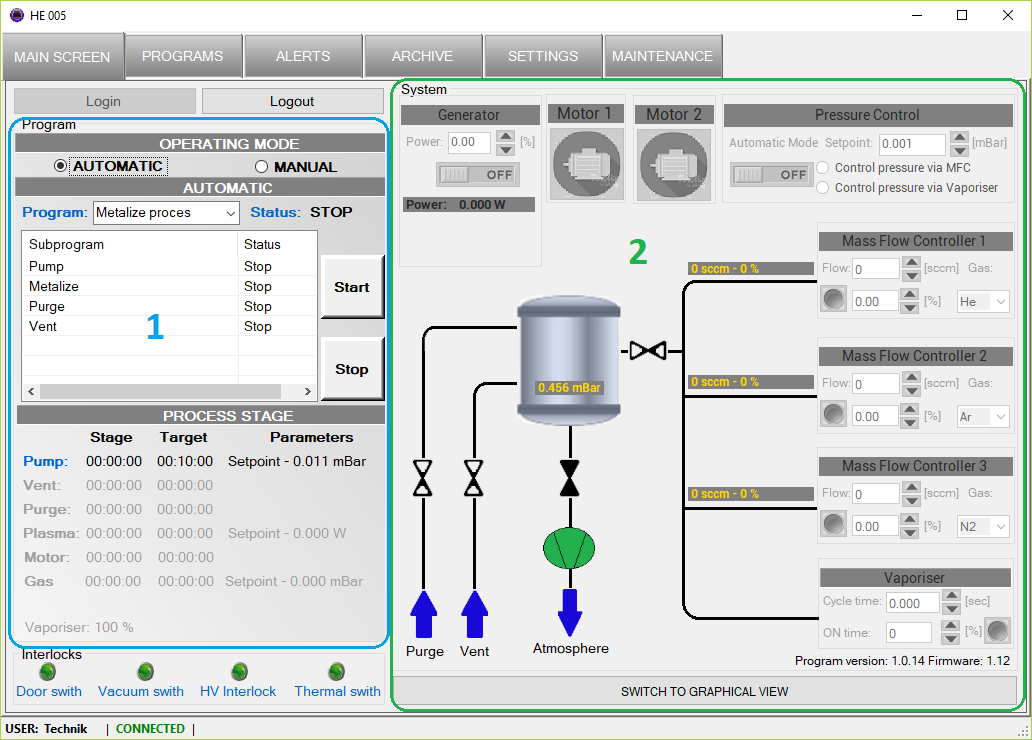
\includegraphics[width=0.7\textwidth]{Graphic/MainScreen/MainScreen.png}	
	\caption{Tab main screen}
	\label{tab_main_screen}
	\end{figure}
	\FloatBarrier

Tab was divided  on two section:

\begin{itemize}
	\item \textit{ Program} - displays information about running program and give possibility to control of process
	\item \textit{ System} - contain all informations about system. There are we can find information about: state of fore pump and  valves,  gas flow, state of power supply  and motors, value of pressure  in chamber 
\end{itemize}

In addition, we will find information on the important signals of the machine. Section \ textit {Interlocks} inform us about the pressure in the chamber, the overheating of  chamber, state of door and conditions of envirment for switches on the power supply.

\begin{itemize}
	\item \textit{Door switch} - state of chamber door. Interlock light when door is closed. 
	\item \textit{Vacuum swith} - state of vacuum switch signal which inform us about pressure in chamber. Interlock light  when pressure is lower than set threshold
	\item \textit{HV Interlock} - state of protection signal power supply against turned on it in dangerouse envirment. Interlock light when pressure is lower than limit, vacuum swtich is OK and system is not overheated (Interlock thermal switch light)
	\item \textit{Thermal swith} - inform us about overhead of chamber. When chamber is overhead signal is not light
\end{itemize}

	\begin{figure}[!h] 
	\centering 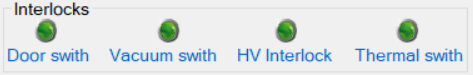
\includegraphics[width=0.5\textwidth]{Graphic/MainScreen/Interlocks.png}	
	\caption{Interlocks}
	\label{interlocks}
	\end{figure}
	\FloatBarrier

Machine, in dependency of privileges of user, can be controlled in one of  below operation mode:

\begin{itemize}
	\item Automatic
	\item Manual
\end{itemize}

\subsection{Automatic mode}

Automatic mode allows us execute a sequence of operations earlier defined. Defined operations contains some parameterized actions which controlled machine. In order to controlled machine by one of defined operation we should select one of program and load him to machine by click button \textit{Start}

	\begin{figure}[!h] 
	\centering 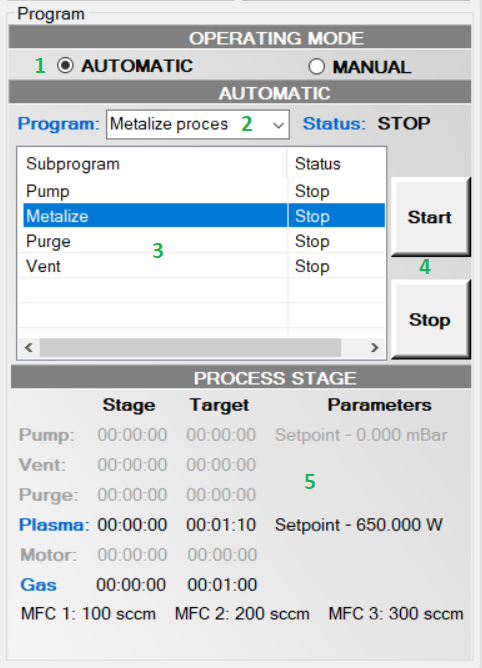
\includegraphics[width=0.4\textwidth]{Graphic/MainScreen/AutomaticMode.png}	
	\caption{Automatic mode}
	\label{automatic_mode}
	\end{figure}
	\FloatBarrier

Above picture displays the section of the application which is responsible for the controlled operation mode as \textit{Automatic Mode}
From this section we can do:

\begin{enumerate}
	\item Choose operating mode as \textit{Automatic}
	\item Choose program to load in machine
	\item Select subprogram to check  it parameters
	\item See of information about selected subprogram:
	\begin{itemize}
		\item \textit{Stage} - actual time executing a stage
		\item\textit{Target} - maximum  time of executing a stage
		\item \textit{Parameters} - view of parameters of current stage
	\end{itemize}
\end{enumerate}

\subsection{Manual mode}

Manual mode allows us control each devices of system separately

	\begin{figure}[!h] 
	\centering 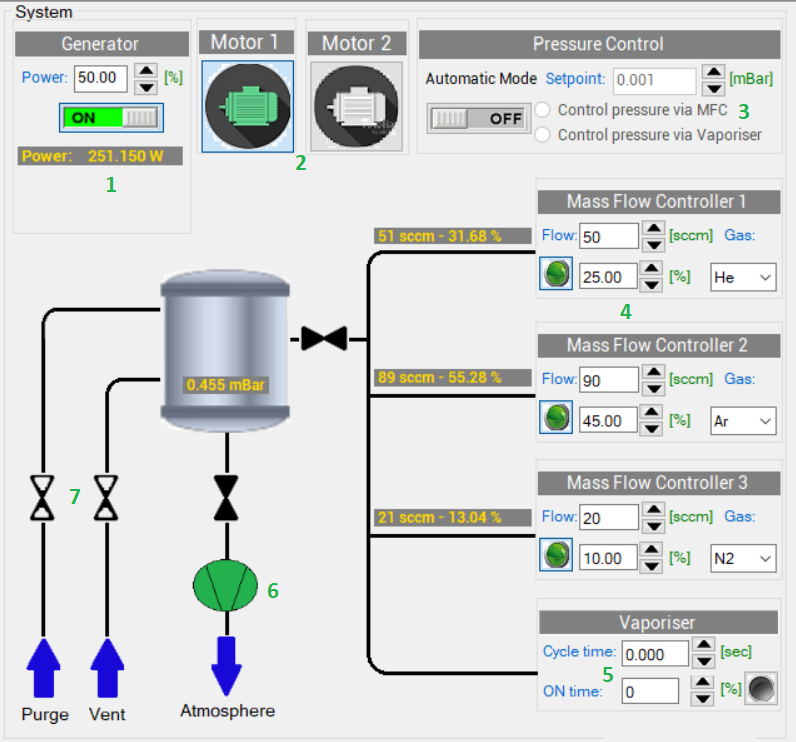
\includegraphics[width=0.6\textwidth]{Graphic/MainScreen/ManualMode.png}	
	\caption{System view}
	\label{system_view}
	\end{figure}
	\FloatBarrier

We can control manually below devices:

	\begin{enumerate}
		\item  Generator - can turn on power supply on set value percent of power
		\item  Motor - can turn on / turn of 
		\item  Pressure control - can set mode of pressure of chamber as automatic that mean we set only value
			of pressure what is should be held in chamber by flow of gases via Mass Flow Controller or Vaporiser
		\item Mass Flow Controller - can set target of flow gas and type gas which is currently connected to MFC
		\item Vaporaiser - can set parameters of vaporiser: cycle time and time opening during a cycle time or count of shot per minute
	   \item Fore pump - can turn on / turn of fore pump
	  \item Valves - by click on corresponding  valves we can open/close him

	\end{enumerate}

\subsection{Graphical view}

\textit{Graphical view} displays on live values from the sensors of system as plot. We see actually value of sensors and value from past. Range time of  values from the past could be defined by user in tab \textit{Settings} by change parameter \textit{Chart window}. 

	\begin{figure}[!h] 
	\centering 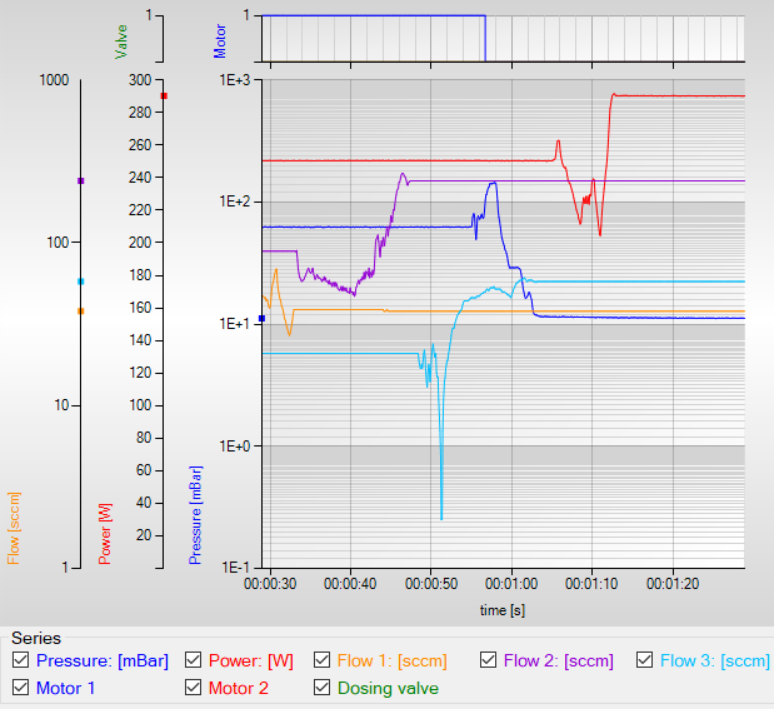
\includegraphics[width=0.57\textwidth]{Graphic/MainScreen/Chart.png}	
	\caption{Graphical view}
	\label{graphical_view}
	\end{figure}
	\FloatBarrier

On chart can we read below values:
\begin{itemize}
\item pressure from pressure gauge
\item power of power supply
\item flow of all mass flow controller
\item state of motors
\item state of dosing valve
\end{itemize} 

Switching between \textit{Graphical view} and \textit{System view} we do by buttons:
\begin{itemize}
\item pressure from pressure gauge
\item power of power supply
\end{itemize} 

	\begin{figure}[!h] 
	\centering 
\includegraphics[width=0.6\textwidth]{Graphic/MainScreen/BtnSwithToGraphicalView.png}	
	\caption{Button switch to graphical view}
	\label{button_switch_to_graphical_view}
	\end{figure}
	\FloatBarrier

	\begin{figure}[!h] 
	\centering 
\includegraphics[width=0.6\textwidth]{Graphic/MainScreen/BtnSwithToMIMC.png}	
	\caption{Button switch to system view}
	\label{Button_switch_to_ system_view}
	\end{figure}
	\FloatBarrier


